\nxsection{Les Cat\'egories d'Articles}
\index{les cat\'egories d'articles}

\nxsubsection{Afficher les d\'etails d'une cat\'egorie d'articles}
\index{afficher les d\'etails d'une cat\'egorie d'articles}
\index{d\'etails d'une cat\'egorie d'articles}

\begin{figure}[!htpb]
	\centering
	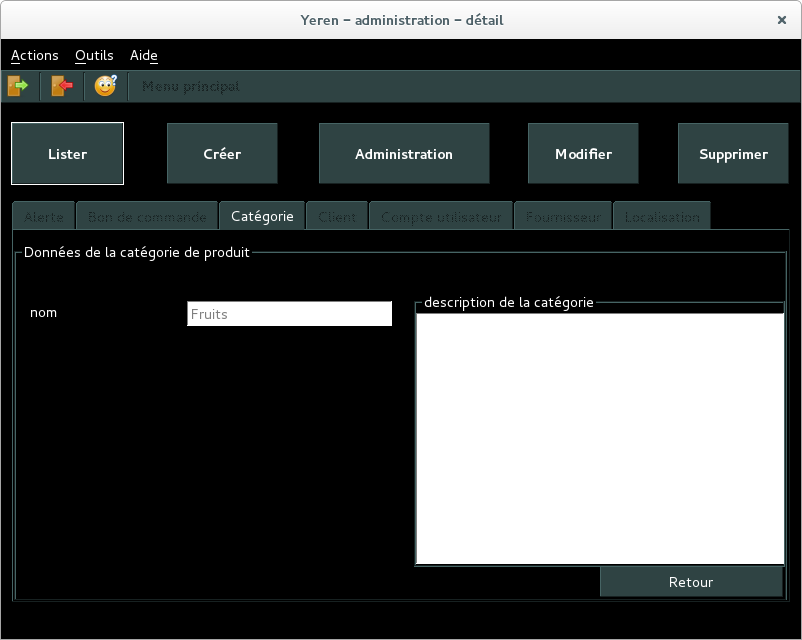
\includegraphics[scale=0.45]{images/categorie-articles-afficher-details.png}
	\caption{L'interface graphique pour afficher les d\'etails d'une
			cat\'egorie d'articles.}
	\label{fig:admin-categories-articles-afficher-details}
\end{figure}

La figure~\ref{fig:admin-categories-articles-afficher-details}
illustre l'interface graphique de \yeren qui affiche
les d\'etails d'une cat\'egorie d'articles.

\procparagraph{Proc\'edure pour afficher les d\'etails
	d'une cat\'egorie d'articles}
\begin{enumerate}[1)]
	\item \`A partir de l'interface graphique de l'acceuil de
		l'administration (voir figure~\ref{fig:fenetre-administrateur}),
		on clique sur l'onglet intitul\'e \textbf{op\'erations}. 
		
	\item Choisir '\textbf{lister}' dans le '\emph{combo box
		op\'erations}'.
		
	\item Choisir '\textbf{une cat\'egorie d'articles}' dans le
		'\emph{combo box objets}'. Vous \^etes automatiquement
		conduit \`a la fen\^etre illustr\'ee par la
		figure~\ref{fig:admin-categories-articles-lister}.
		
	\item S\'electionner la cat\'egorie d'articles dont vous
		souhaitez afficher les d\'etails.
		
	\item Cliquer sur le bouton \bouton{Afficher}. Les d\'etails
		sur la cat\'egorie d'articles sont affich\'es dans une
		nouvelle fen\^etre.
\end{enumerate}

%%%%%%%%%%%%%%%%%%%%%%%%%%%%%%%%%%%%%%%%%%%%%%%%%%%%%%%%%%%%%%%%%%%%%%%%%%%%%%%%%

\newpage
\nxsubsection{Cr\'eer une cat\'egorie d'articles}
\index{cr\'eer une cat\'egorie d'articles}

\begin{figure}[!htpb]
	\centering
	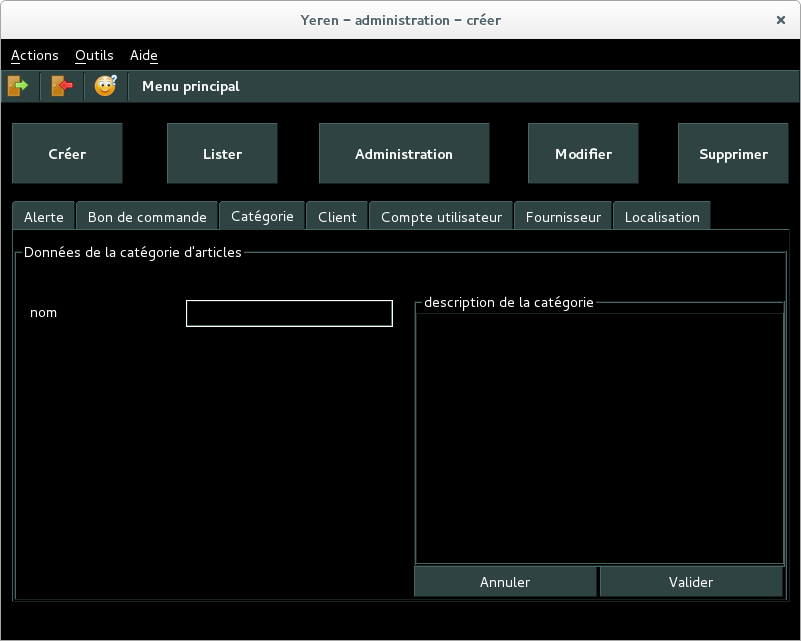
\includegraphics[scale=0.45]{images/categorie-articles-creer.png}
	\caption{L'interface graphique pour cr\'eer une cat\'egorie d'articles.}
	\label{fig:admin-categories-articles-creer}
\end{figure}

La figure~\ref{fig:admin-categories-articles-creer} illustre
l'interface graphique de \yeren pour cr\'eer une nouvelle
cat\'egorie d'articles.

\procparagraph{Proc\'edure pour cr\'eer une cat\'egorie d'articles}
\begin{enumerate}[1)]
	\item \`A partir de l'interface graphique de l'acceuil de
		l'administration (voir figure~\ref{fig:fenetre-administrateur}),
		on clique sur l'onglet intitul\'e \textbf{op\'erations}. 
		
	\item Choisir '\textbf{cr\'eer}' dans le '\emph{combo box
		op\'erations}'.
		
	\item Choisir '\textbf{une cat\'egorie d'articles}' dans
		le '\emph{combo box objets}'. Vous \^etes automatiquement
		conduit \`a la fen\^etre illustr\'ee par la
		figure~\ref{fig:admin-categories-articles-creer}.
		
	\item Saisissez la d\'esignation de la nouvelle cat\'egorie
		d'articles \`a cr\'eer dans le champs de texte
		'\textbf{d\'esignation}'.

	\item Si vous le souhaitez, saisisser un texte qui d\'ecrit
		cette nouvelle cat\'egorie d'articles dans le champs de
		texte '\textbf{description de la cat\'egorie}'.
		
	\item Cliquer sur le bouton \bouton{Valider} pour
		valider votre travail.		
\end{enumerate}

%%%%%%%%%%%%%%%%%%%%%%%%%%%%%%%%%%%%%%%%%%%%%%%%%%%%%%%%%%%%%%%%%%%%%%%%%%%%%%%%%

\newpage
\nxsubsection{Lister les cat\'egories d'articles}\label{sec:administration-categorie-lister}
\index{lister les cat\'egories d'articles}

\begin{figure}[!htpb]
	\centering
	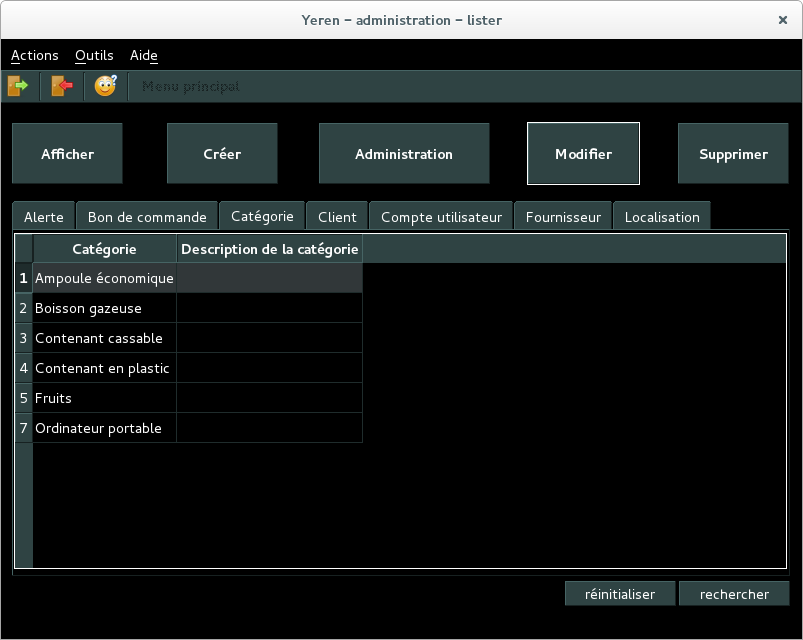
\includegraphics[scale=0.45]{images/categorie-articles-lister.png}
	\caption{L'interface graphique qui liste les cat\'egories d'articles.}
	\label{fig:admin-categories-articles-lister}
\end{figure}

La figure~\ref{fig:admin-categories-articles-lister} illustre
l'interface graphique de \yeren qui liste les cat\'egories
d'articles.

\procparagraph{Proc\'edure pour lister les cat\'egories d'articles}
\begin{enumerate}[1)]
	\item \`A partir de l'interface graphique de l'acceuil de
		l'administration (voir figure~\ref{fig:fenetre-administrateur}),
		on clique sur l'onglet intitul\'e \textbf{op\'erations}. 
		
	\item Choisir '\textbf{lister}' dans le '\emph{combo box
		op\'erations}'.
		
	\item Choisir '\textbf{une cat\'egorie d'articles}' dans
		le '\emph{combo box objets}'. Vous \^etes automatiquement
		conduit \`a la fen\^etre qui liste les cat\'egories
		d'articles (figure~\ref{fig:admin-categories-articles-lister}).
\end{enumerate}

%%%%%%%%%%%%%%%%%%%%%%%%%%%%%%%%%%%%%%%%%%%%%%%%%%%%%%%%%%%%%%%%%%%%%%%%%%%%%%%%%

\newpage
\nxsubsection{Modifier les d\'etails d'une cat\'egorie d'articles}
\index{modifier les d\'etails d'une cat\'egorie d'articles}

\begin{figure}[!htpb]
	\centering
	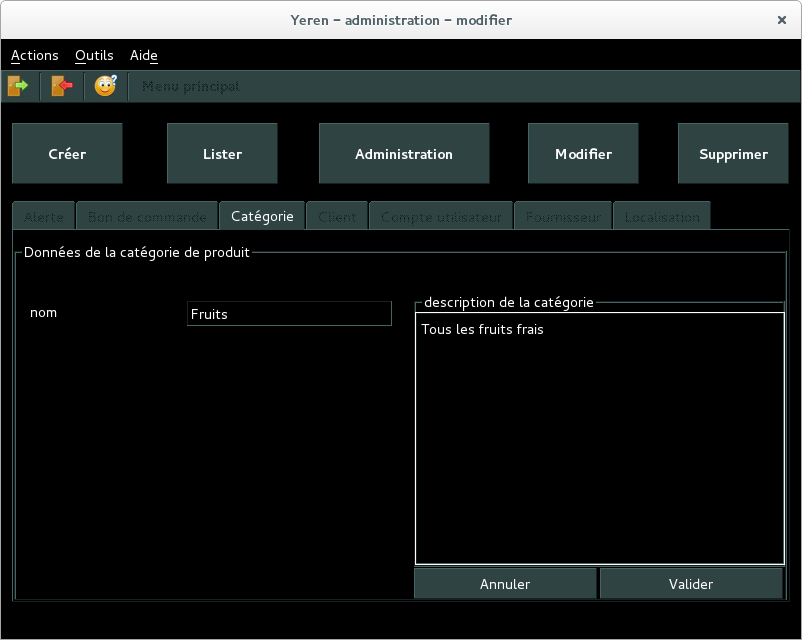
\includegraphics[scale=0.45]{images/categorie-articles-modifier.png}
	\caption{L'interface graphique pour modifier les d'\'etails
			d'une cat\'egorie d'articles.}
	\label{fig:admin-categories-articles-modifier}
\end{figure}

La figure~\ref{fig:admin-categories-articles-modifier}
illustre l'interface graphique de \yeren pour modifier
les d\'etails d'une cat\'egorie d'articles.

\procparagraph{Proc\'edure pour modifier les d\'etails
	d'une cat\'egorie d'articles}
\begin{enumerate}[1)]
	\item \`A partir de l'interface graphique de l'acceuil de
		l'administration (voir figure~\ref{fig:fenetre-administrateur}),
		on clique sur l'onglet intitul\'e \textbf{op\'erations}. 
		
	\item Choisir '\textbf{lister}' dans le '\emph{combo box
		op\'erations}'.
		
	\item Choisir '\textbf{cat\'egorie d'articles}' dans le
		'\emph{combo box objets}'. Vous \^etes automatiquement
		conduit \`a la fen\^etre illustr\'ee par la
		figure~\ref{fig:admin-categories-articles-lister}.
		
	\item S\'electionner l'alerte dont vous souhaitez modifier
		les d\'etails dans la liste	des d\'esignations des
		cat\'egories d'articles affich\'ee.
		
	\item Cliquer sur le bouton \bouton{Modifier}. Les d\'etails
		sur le stock sont affich\'es dans une nouvelle fen\^etre.
		
	\item Faites les modifications que vous souhaitez. Pour
		les alertes, seul le message d'alerte peut \^etre
		modifi\'e.
		
	\item Cliquer sur le bouton \bouton{valider} pour valider
		les modifications faites.
\end{enumerate}

%%%%%%%%%%%%%%%%%%%%%%%%%%%%%%%%%%%%%%%%%%%%%%%%%%%%%%%%%%%%%%%%%%%%%%%%%%%%%%%%%

\newpage
\nxsubsection{Supprimer une cat\'egorie d'article}
\index{supprimer une cat\'egorie d'article}

\begin{figure}[!htpb]
	\centering
	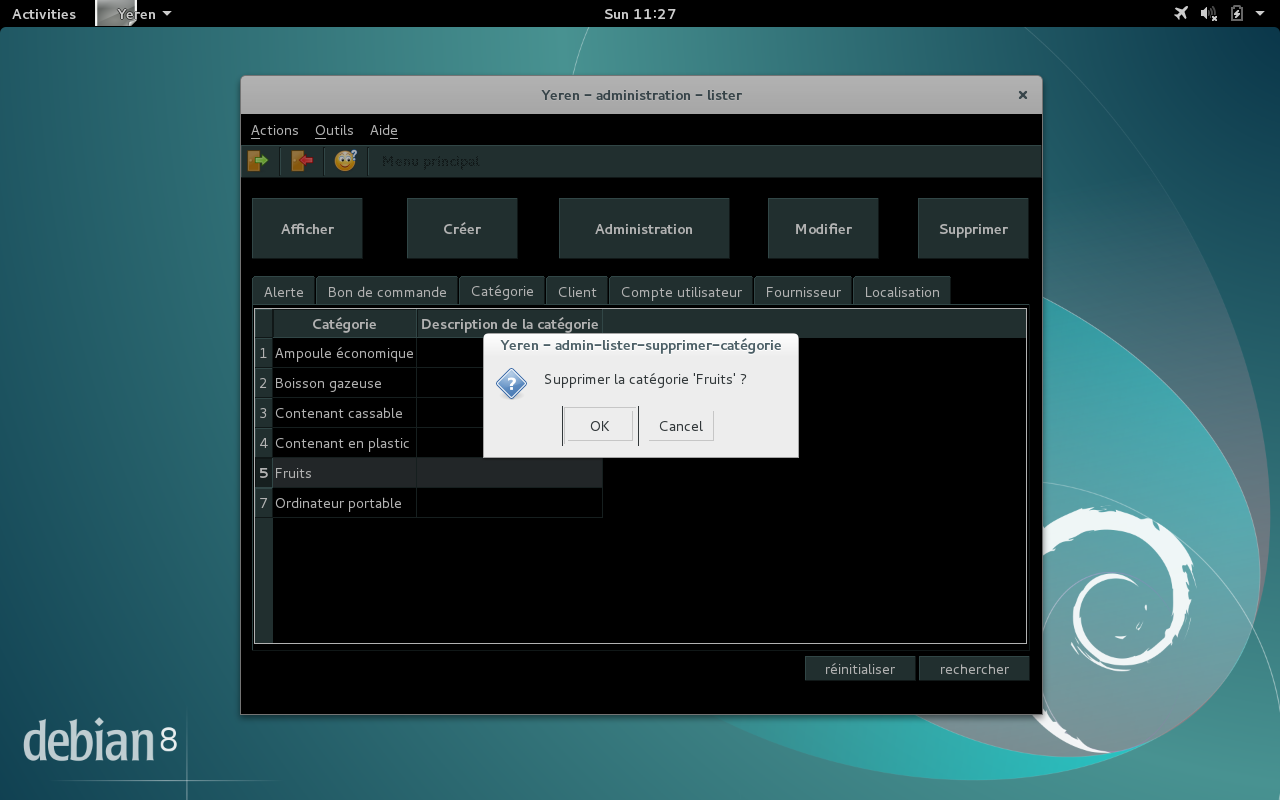
\includegraphics[scale=0.39]{images/categorie-articles-supprimer.png}
	\caption{L'interface graphique pour supprimer une cat\'egorie d'articles.}
	\label{fig:admin-categories-articles-supprimer}
\end{figure}

La figure~\ref{fig:admin-categories-articles-supprimer} illustre
l'interface graphique de \yeren pour supprimer une
cat\'egorie d'articles.

\procparagraph{Proc\'edure pour supprimer une cat\'egorie d'articles}
\begin{enumerate}[1)]
	\item \`A partir de l'interface graphique de l'acceuil de
		l'administration (voir figure~\ref{fig:fenetre-administrateur}),
		on clique sur l'onglet intitul\'e \textbf{op\'erations}. 
		
	\item Choisir '\textbf{supprimer}' dans le '\emph{combo box
		op\'erations}'.
		
	\item Choisir '\textbf{une cat\'egorie d'articles}' dans le
		'\emph{combo box objets}'. Vous \^etes automatiquement
		conduit \`a la fen\^etre illustr\'ee par la
		figure~\ref{fig:admin-categories-articles-lister}.
		
	\item S\'electionner l'alerte \`a supprimer dans la liste
		des d\'esignations des cat\'egories d'articles affich\'ee.
		
	\item Cliquer sur le bouton \bouton{Supprimer}. La question
		est ensuite pos\'ee si vous confirmer votre choix.
		Cliquer sur le \bouton{OK} pour confirmer votre choix.
\end{enumerate}
